\documentclass[Kravspecifikation/Kravspec_Main.tex]{subfiles}
\begin{document}


\section{Ikke-funktionelle krav}\label{sec:ikke_funktionelle_krav}
De ikke funktionelle krav beskriver systemets fysiske dimensioner, fysiske parameter, og det forskellige GUI. Herudover beskriver det også en række specifikationer om systemet ydeevne. For specifik forklaring, se Definitionsliste (side xx).

Til at beskrive nogle af kravene er der nogle skitser som hjælper med at forklare kravene. 
\subsection{Fysiske Parametre}
Dimensioner bliver angivet i følgende format [længde/bredde/højde][cm]
\refstepcounter{req}
\begin{table}[H]
\centering
\begin{tabular}{|L{0.1\textwidth}|L{0.6\textwidth}|L{0.15\textwidth}|}
\hline
\textbf{ID} & \textbf{Krav} & \textbf{Prioritet} \\ \hline
\subreq{} \label{req:table-dimensions} & Beer Pong bordet skal være 240cm/60cm/70cm +/- 1cm  &  C\\ \hline
\subreq{} \label{req:ball-size} & Systemet skal kunne håndtere en \textbf{Ball} med en diameter på 40mm +/- 1mm & M  \\ \hline
\subreq{} \label{req:display-size} & Display'ets billede skal være 24 tommer +/- 0.5 tommer diagonalt med et format på 16:9 med en opløsning på 1920x1080& S \\ \hline
\subreq{} \label{req:cup-size} & Systemet skal kunne håndtere \textbf{Cups} med en øvre diameter på $94\si{mm} \pm 3\si{mm}$ og en nedre diameter på $65\si{mm} \pm 3\si{mm}$ og en højde på $120mm \pm{5mm}$ & M\\ \hline
\subreq{} \label{req:coin-size} & Systemet skal kun acceptere en dansk femkrone\autocite{fiveKrCoin} som betaling. Diameter på 28.5 mm +/- 0.5mm og tykkelse på 2.00 +/- 0.1 mm & M\\ \hline
\subreq{} \label{req:coin-max-size}& Systemet skal frigive \textbf{Coins} med en diameter på 28.0 mm og under og tykkelse på 2.35 mm og under & M\\ \hline
\subreq{} \label{req:light-D-inner}& $D_{inner}$ på figur \ref{fig:LEDplacement} skal være $55\si{mm} \pm 1\si{mm}$  & S \\ \hline
\subreq{} \label{req:light-D-center}& $D_{center}$ på figur \ref{fig:LEDplacement} skal være $65\si{mm} \pm 1\si{mm}$  & S \\ \hline
\subreq{} \label{req:light-D-led} & $D_{led}$ på figur \ref{fig:LEDplacement} skal være $5\si{mm} \pm 1\si{mm}$  & S \\ \hline
\subreq{} \label{req:light-D-outer}& $D_{outer}$ på figur \ref{fig:LEDplacement} skal være $75\si{mm} \pm 1\si{mm}$   & S \\ \hline
\subreq{} \label{req:light-led-angle}& Vinklen mellem to LED'er i \textit{\textbf{Cup light}} skal være $70^{\circ} \pm 2^{\circ}$ & S \\ \hline
\subreq{} \label{req:cup-holder-distance} & Afstanden mellem centrum for to \textit{\textbf{Cupholders}} skal være $100\si{mm} \pm 2\si{mm}$ & M \\ \hline
\subreq{} \label{req:beer-amount}& Systemet skal fungere med $110\si{ml} \pm 20\si{ml}$ Ceres Top øl i hver \textbf{Cup} & M\\ \hline
\subreq{} \label{req:ball-color} & Systemet skal fungere med en hvid \textbf{Ball} & M\\ \hline
\subreq{} \label{req:ball-drop-height} & Systemet skal detektere en \textbf{Ball} der falder fra en højde på $30\si{cm} \pm 1\si{cm}$ over bordet. & S\\ \hline 
\subreq{} \label{req:max-cup-offset} & Systemet skal detektere placering af en \textbf{Cup} når afstanden mellem centrum af \textbf{Cup} og centrum af \textit{\textbf{Cupholder}} er under 10mm & M\\ \hline
\subreq{} \label{req:ball-dispenser-full-amount} & \textit{\textbf{Ball dispenser}} skal kunne indeholde 14 \textbf{Balls}. & S\\ \hline
\end{tabular}
\caption{Ikke funktionelle krav for de fysiske dimensioner}
\label{tab:fysiske_dimensioner}
\end{table}


\subsection{User Interface}
Der er til de forskellige dele af \textit{\textbf{UI}}, lavet skitser der forklare hvilke elementer der skal være, samt placeringen og dimensionerne for disse elementer.
\subsubsection{Cupholder}
Der er lavet en skitse der beskriver hvordan en \textit{\textbf{Cupholder}} ser ud. Dette kan ses på figur \ref{fig:LEDplacement}

\begin{figure}[H]
    \centering
    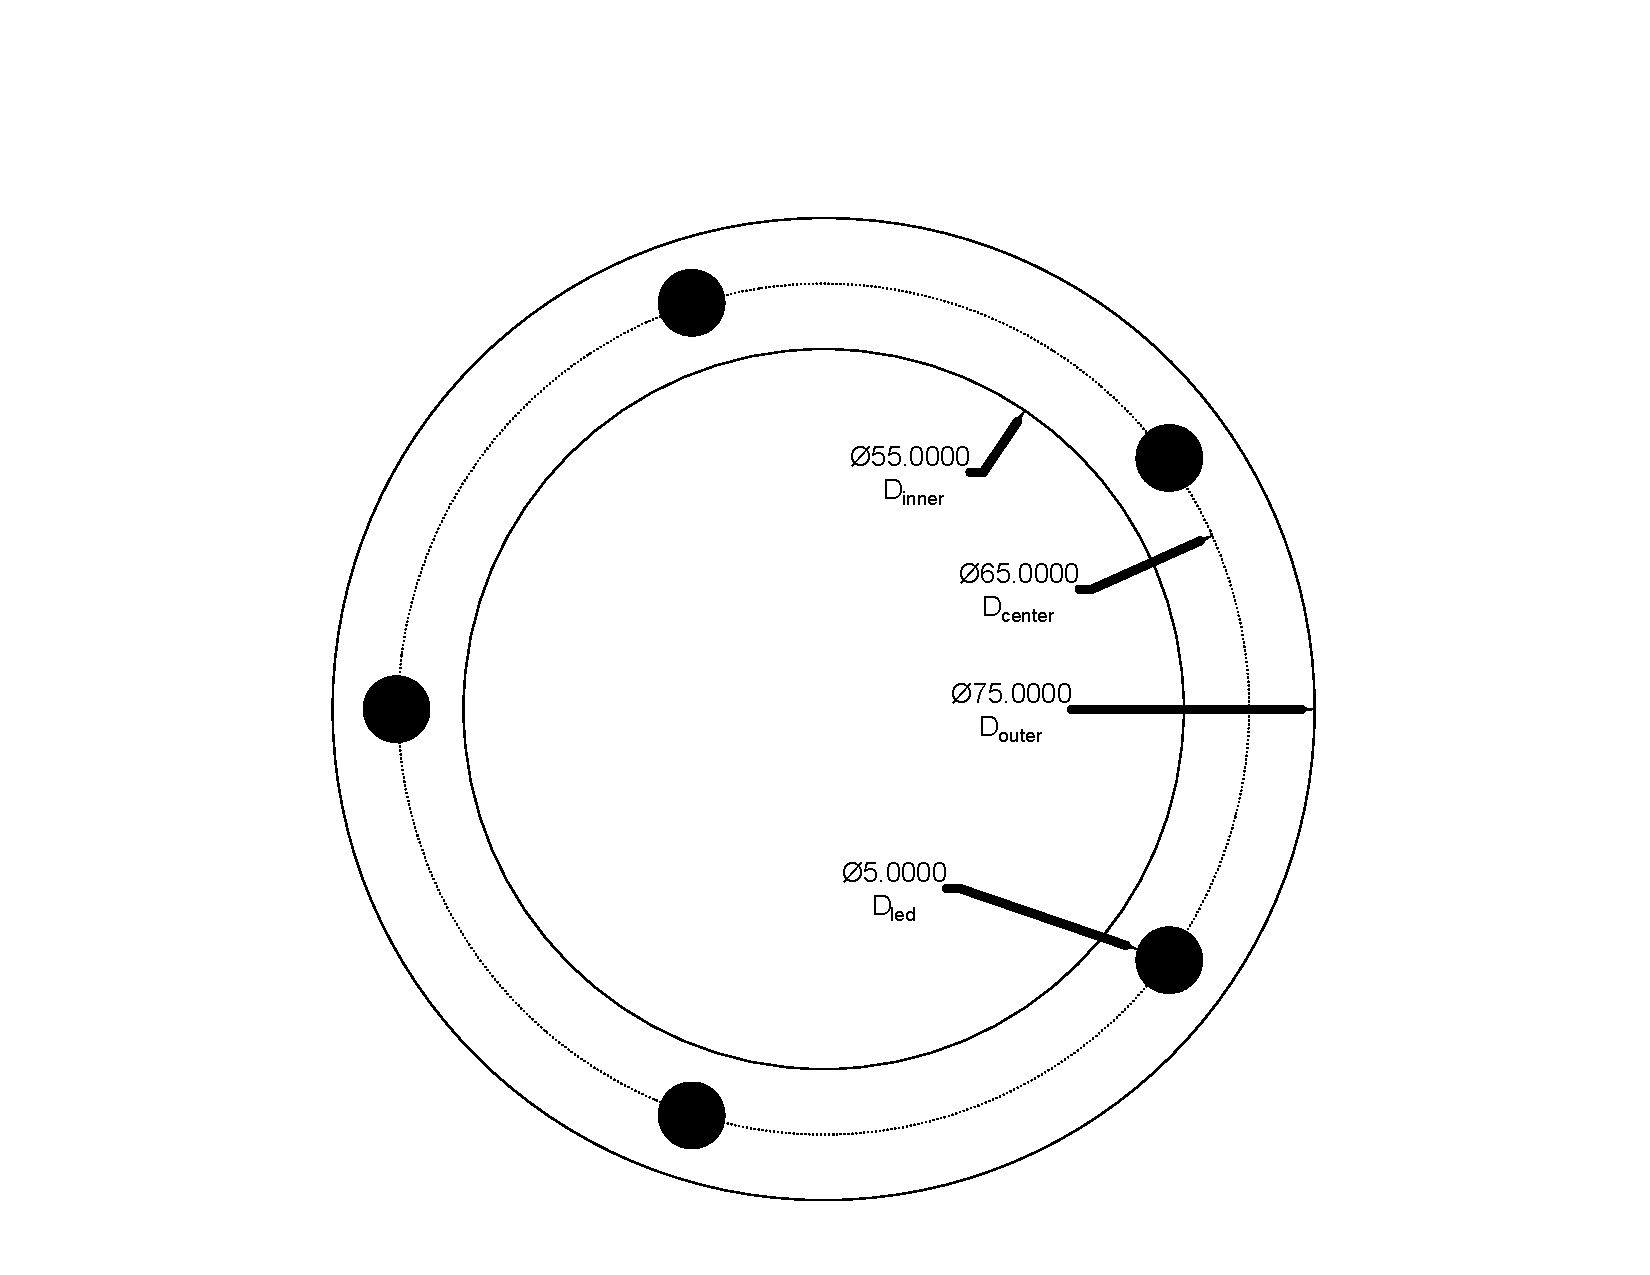
\includegraphics[width=0.8\textwidth,trim={2in 0.4in 2in 1.3in},clip, page=1]{Kravspecifikation/Ikke-funktionelle/graphics/LEDplacement.pdf}
    \caption{Skitse der viser de forskellige dele af en \textit{\textbf{Cupholder}}. Der er påtegnet forskellige diametre med mål. Målenes tolerance er specificeret i tabel \ref{tab:fysiske_dimensioner}.}
    \label{fig:LEDplacement}
\end{figure}

På figur \ref{fig:LEDplacement} er der en ring af lys (\textit{\textbf{Cup light}}). Denne ring er afgrænset af den indre cirkel (med diameteren $D_{inner}$ og den ydre cirkel (med diameteren $D_{outer}$). De 5 sorte cirkler (med diameteren $D_{led}$) repræsenterer LED'er som er lyskilderne i \textit{\textbf{Cup light}}. De er placeret på en cirkel med diameteren $D_{center}$. LED'ernes placering $(D_{led})$ er valgt ud fra at passe med de fysiske krav på en \textbf{Cup} (se krav i ).
\refstepcounter{req}

\subsubsection{WebPage}
\begin{figure}[H]
    \centering
    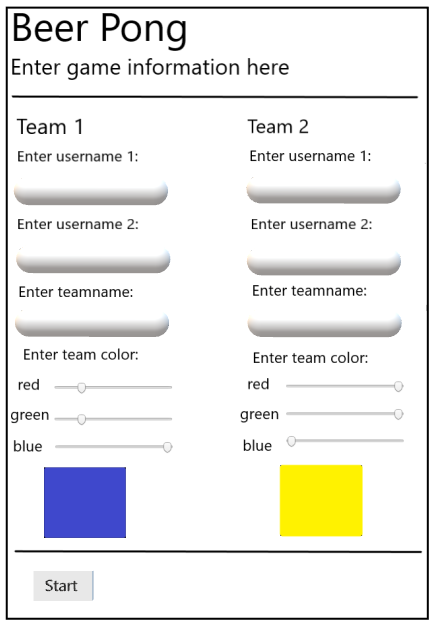
\includegraphics[width=0.6\textwidth]{Kravspecifikation/Ikke-funktionelle/graphics/WebPage_IF.png}
    \caption{Skitse af grænsefladen for WebPage}
   \label{fig:WebPage_IF}
\end{figure}

\begin{table}[H]
\centering
\begin{tabular}{|L{0.1\textwidth}|L{0.65\textwidth}|L{0.15\textwidth}|}
\hline
\textbf{ID} & \textbf{Krav} & \textbf{Prioritet} \\ \hline
\subreq{} \label{req:wifi-name}& Systemet skal hoste et wifi netværk med SSID ''Beer\_Pong\_Table'' og adgangskoden ''beerpong''. & S\\ \hline
\subreq{} \label{req:led-same-color} & De fem LED'er i \textit{\textbf{Cup light}} til en \textit{\textbf{Cupholder}} skal lyse med den samme farve. & M\\ \hline
\subreq{} \label{req:color-count} & Et enkelt \textit{\textbf{Cup light}} skal kunne lyse med mindst 10 forskellige farver & M\\ \hline
\subreq{} \label{req:color-control} & Hvert \textit{\textbf{Cup light}} skal kunne styres individuelt & M\\ \hline 
\subreq{} \label{req:missing-cup-color} & Et \textit{\textbf{Cup light}} skal i UC1 lyse gul når der ikke er en \textbf{Cup} i den tilhørende \textit{\textbf{Cupholder}}  & S\\ \hline
\subreq{} \label{req:placed-cup-color} & Et \textit{\textbf{Cup light}} skal i UC1 lyse blå når der er en \textbf{Cup} i den tilhørende \textbf{Cup} holder & S\\ \hline
\subreq{} \label{req:status-colors} & Lysdioderne på \textit{\textbf{Ball dispenser status lights}} skal lyse i hver deres farve, rød og grøn & M \\ \hline
\subreq{} \label{req:status-empty-light} & Den røde lysdiode i \textit{\textbf{Ball dispenser status lights}} skal lyse, når der er færre end to \textbf{Balls} tilbage i \textit{\textbf{Ball dispenser}} & M \\ \hline
\subreq{} \label{req:status-full-light}& Den grønne lysdiode i \textit{\textbf{Ball dispenser status lights}} skal lyse, når \textit{\textbf{Ball dispenser}} er fuld af \textbf{Balls} som specificeret i krav K\ref{req:ball-dispenser-full-amount} & M  \\ \hline
\subreq{} \label{req:webpage-address} & WebPage er en hjemmeside med statisk IP-adresse 10.9.8.2., som er hostet af systemet & S\\ \hline
\subreq{} \label{req:webpage-language} & Alt tekst på WebPage skal være på sproget engelsk. & M\\ \hline
\subreq{} \label{req:webpage-info-type} & På WebPage skal der for hvert af de to hold indtastes følgende \textit{\textbf{spiller oplysninger}}: \textit{teamname}, \textit{username1} og \textit{username2}. & M\\ \hline
\subreq{} \label{req:webpage-string-length} & Holdnavne og brugernavne indtastet på WebPage skal være tekststrenge, med en længde på mellem 1 og 15 karakterer. & M\\ \hline
\subreq{} \label{req:webpage-color-select} & På WebPage skal der for hvert af de to hold kunne vælges følgende \textit{\textbf{spiller oplysninger}}: \textbf{holdfarve}, ved at justere intensiteten af farverne rød, grøn og blå i et RGB farveskema. & S\\ \hline
\subreq{} \label{req:webpage-color-size} & Der skal kunne vælges mindst 10 forskellige farver på WebPage. & S\\ \hline
\subreq{} \label{req:GUI-language}& Alt tekst på GUI skal være på sproget engelsk. & M \\ \hline
\subreq{} \label{req:GUI-info-type} & På GUI skal der for hvert af de to hold vises \textit{\textbf{spiller oplysninger}}: \textit{teamname}, \textit{username1} og \textit{username2}. & M\\ \hline
\end{tabular}
\caption{Ikke funktionelle krav for User Interface}
\label{tab:user_interface}
\end{table}

\subsection{Ydeevne}

\refstepcounter{req}
\begin{table}[H]
\centering
\begin{tabular}{|L{0.1\textwidth}|L{0.65\textwidth}|L{0.15\textwidth}|}
\hline
\textbf{ID} & \textbf{Krav} & \textbf{Prioritet} \\ \hline
\subreq{} \label{req:ball-response-time} & Den første \textbf{Ball} skal have forladt \textit{\textbf{Ball dispenser}} indenfor 5s efter der indsættes en \textbf{Coin}. &  S\\ \hline
\subreq{} \label{req:won-response-time} & Når den sidste \textbf{Cup} er fjernet fra sin \textbf{\textit{Cupholder}}, \textbf{\textit{Display}} vise, hvem der har vundet indenfor 500 ms. &  M\\ \hline
\subreq{} \label{req:waterproof} & Systemet skal være stænktæt. Dvs. øl, sodavand og andet væske ikke kan komme til systemet indre sensorer eller computer. &  S\\ \hline

\subreq{} \label{req:startup-turnon-time} & Systemets \textbf{\textit{start op}} tid skal være mindre end 10s. & M \\ \hline
\subreq{} \label{req:startup-turnoff-time} & Systemets \textbf{\textit{slukke}} tid skal være mindre end 10 sekunder. & M \\ \hline
\subreq{} \label{req:remove-cup-response-time} & \textit{\textbf{Display}} skal vise at en person har fjernet et \textbf{Cup} fra en \textit{\textbf{Cupholder}} indenfor 500ms. & M \\ \hline
\subreq{} \label{req:max-start-time} & Fra der trykkes 'Start' på WebPage til at \textbf{\textit{Cup light}} opdateres må der som maksimum gå 1s. &  M\\ \hline
\end{tabular}
\caption{Ikke funktionelle krav for ydeevne}
\label{tab:ydeevne}
\end{table}

\subsection{Pålidelighed}
\refstepcounter{req}
\begin{table}[H]
\centering
\begin{tabular}{|L{0.1\textwidth}|L{0.65\textwidth}|L{0.15\textwidth}|}
\hline
\textbf{ID} & \textbf{Krav} & \textbf{Prioritet} \\ \hline
\subreq{} \label{req:placed-succes-rate} & Det skal detekteres 99 ud af 100 gange at der placeres en \textbf{Cup} i en \textit{\textbf{Cupholder}}.  & M \\ \hline
\subreq{} \label{req:removed-succes-rate} & Det skal detekteres 99 ud af 100 gange at der løftes en \textbf{Cup} fra en \textit{\textbf{Cupholder}}.  & M \\ \hline
\subreq{} \label{req:dropped-succes-rate} & Det skal detekteres 95 ud af 100 gange at en \textbf{Ball} rammer i  en \textbf{Cup} som står i en \textit{\textbf{Cupholder}}. & S \\ \hline
\subreq{} \label{req:hour-false-placed} & I en periode på 1 time må der højest være 1 falsk detektering af placering af en \textbf{Cup} på tom \textit{\textbf{Cupholder}} & M \\ \hline
\subreq{} \label{req:hour-false-removed}& I en periode på 1 time må der højest være 1 falsk detektering af løfting af en \textbf{Cup} fra \textit{\textbf{Cupholder}} hvor der står en \textbf{Cup}& M \\ \hline
\subreq{} \label{req:ball-hit-sensor-false-placed} & Når en \textbf{Ball} rammer en \textit{\textbf{Cupholder}} og hopper væk igen 100 gange (uden nogen \textbf{Cup}) må der højest ske 1 falsk detektering af at der placeres en \textbf{Cup} i den givne \textit{\textbf{Cup holder}}& M \\ \hline
\subreq{} \label{req:inserted-coin-succes-rate} & Det skal detekteres mindst 98 ud af 100 gange at der indsættes en 5 krone i bolddispenser. & M \\ \hline
\subreq{} \label{req:inserted-wrong-coin-false-detect} & Det skal detekteres højst 2 ud af 100 gange at der indsættes en 5 krone i bolddispenser når der indsættes enhver anden dansk \textbf{Coin}. & M \\ \hline
\subreq{} \label{req:hour-false-coin} & I en periode på 1 time må der højest være 1 falsk detektering af indsættelse af en dansk 5 krone i bolddispenser & M \\ \hline
\subreq{} \label{req:ball-delivery-error-count} & Der må højst ske en fejl ved levering af 2 \textbf{Balls} (dvs. der leveres færre eller flere end 2 \textbf{Balls}) 1 ud af 50 gange.  & M \\ \hline
\subreq{} \label{req:webpage-error-rate}& Mindst 49 ud af 50 gange, hvor der trykkes 'Start' på WebPage, skal de rigtige \textit{\textbf{spiller oplysninger}} fremgå af display og \textit{\textbf{Cup lights}}. & M\\ \hline
\end{tabular}
\caption{Ikke funktionelle krav for pålidelighed}
\label{tab:reliability}
\end{table}

\end{document}